\documentclass{article}
\title{Eletrostatics}
\author{Serafí Nebot Ginard}
\date{2023}

\usepackage[parfill]{parskip}
\usepackage{hyperref}
\usepackage{amsmath}
\usepackage{tikz}
\usepackage{wrapfig}
\usepackage[a4paper, total={18cm, 20cm}]{geometry}

\begin{document}
\maketitle
\newpage

\tableofcontents
\newpage

\section{Punctual loads}
A punctual load in space will create an electric field towards all surrounding points in space.

\begin{center}
	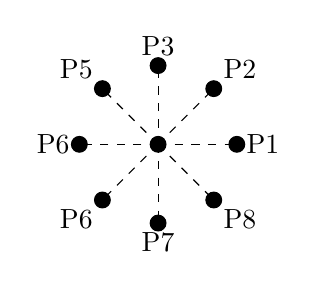
\begin{tikzpicture}
		\coordinate (P0) at (0, 0);
		\coordinate (P1) at +(0:1);
		\coordinate (P2) at +(45:1);
		\coordinate (P3) at +(90:1);
		\coordinate (P4) at +(135:1);
		\coordinate (P5) at +(180:1);
		\coordinate (P6) at +(225:1);
		\coordinate (P7) at +(270:1);
		\coordinate (P8) at +(315:1);

		\filldraw (P0) circle (0.1);
		\filldraw (P1) circle (0.1);
		\filldraw (P2) circle (0.1);
		\filldraw (P3) circle (0.1);
		\filldraw (P4) circle (0.1);
		\filldraw (P5) circle (0.1);
		\filldraw (P6) circle (0.1);
		\filldraw (P7) circle (0.1);
		\filldraw (P8) circle (0.1);

		\draw[-, dashed] (P0) -- (P1) node[right] {P1};
		\draw[-, dashed] (P0) -- (P2) node[above right] {P2};
		\draw[-, dashed] (P0) -- (P3) node[above] {P3};
		\draw[-, dashed] (P0) -- (P4) node[above left] {P5};
		\draw[-, dashed] (P0) -- (P5) node[left] {P6};
		\draw[-, dashed] (P0) -- (P6) node[below left] {P6};
		\draw[-, dashed] (P0) -- (P7) node[below] {P7};
		\draw[-, dashed] (P0) -- (P8) node[below right] {P8};
	\end{tikzpicture}
\end{center}

\begin{wrapfigure}{r}{6cm}
	\vspace{0.5cm}
	\hspace{0.4cm}
	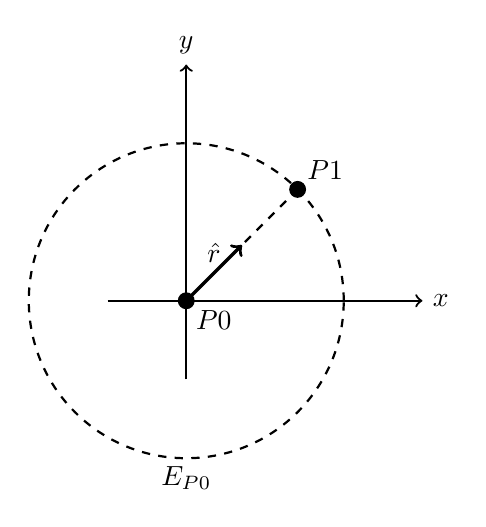
\begin{tikzpicture}
		\coordinate (P0) at (0, 0);
		\coordinate (P1) at +(45:2);

		\filldraw (P0) circle (0.1) node[below right] {$P0$};
		\filldraw (P1) circle (0.1) node[above right] {$P1$};

		\draw[->, thick] (-1, 0) -- (3, 0) node[right] {$x$};
		\draw[->, thick] (0, -1) -- (0, 3) node[above] {$y$};
		\draw[->, dashed, thick] (P0) circle (2);
		\draw[-, dashed, thick] (P0) -- (P1);
		\draw[->, very thick] (P0) -- node[above] {$\hat{r}$} +(45:1);
		\node at +(270:2.25) {$E_{P0}$};
	\end{tikzpicture}
\end{wrapfigure}

In order to measure a punctual load a reference point is needed. For instance, the electric field generated by the punctual load in the center, point $P0$, on point $P1$ is:
\[
	\vec{E}_{P0 \to P1} = k_e\frac{p_0}{r^2}\hat{r}
\]
where $p_0$ is the electric charge at point $P0$ in Coulombs (C), $r$ the
distance between point $P0$ and the reference point $P1$ in meters (m), $\hat{r}$ is the unit vector
indicating the direction of an electric field, and $k_e$ is the Coulomb's constant
\[
	k_e = \frac{1}{4 \pi \epsilon_0} \approx 9 \cdot 10^9
\]
and $\epsilon_0$ is the Vacumm permittivity.

A punctual load also produces a force to all surrounding points in space. The force of an electric
field is written as
\begin{align*}
	\vec{F}_{P0 \to P1} &= p_1 \vec{E}_{P0 \to P1}\\
						&= \frac{1}{4 \pi \epsilon_0} \frac{p_0 p_1}{r^2}\hat{r}
\end{align*}

The unit of an electric force is Newtons ($N$) and the unit of an electric charge is Coulombs ($C$).
Therefore, the unit of an electric field is Netwons/Coulombs ($\frac{N}{C}$).
\begin{align*}
	F = \frac{1}{4 \pi \epsilon_0}\frac{q q'}{r^2} &\Longrightarrow \frac{C^2}{m^2} = N\\
	E = \frac{F}{q} &\Longrightarrow \frac{C^2}{m^2}\frac{1}{C} = \frac{N}{C}
\end{align*}

A punctual load produces an electric potential to all surrounding points in space. The unit of electric potential is Volts ($V$).
\[
	V = \frac{1}{4\pi \epsilon_0}\frac{q}{r} \Longrightarrow \frac{C}{m} = V
\]

\pagebreak
Vectors associated to a punctual load with \emph{positive} charge will point outwards. Vectors
associated to a punctual load with \emph{negative} charge will point inwards.

\begin{figure}[ht]
	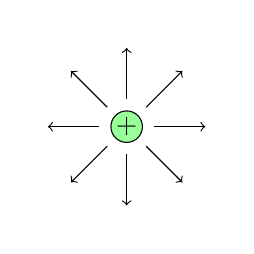
\begin{tikzpicture}
		\filldraw[white] (1.25, 1.25) rectangle (-1.25, -1.25);

		\coordinate (B1) at +(0:1);
		\coordinate (A1) at +(0:0.35);

		\coordinate (B2) at +(45:1);
		\coordinate (A2) at +(45:0.35);

		\coordinate (B3) at +(90:1);
		\coordinate (A3) at +(90:0.35);

		\coordinate (B4) at +(135:1);
		\coordinate (A4) at +(135:0.35);

		\coordinate (B5) at +(180:1);
		\coordinate (A5) at +(180:0.35);

		\coordinate (B6) at +(225:1);
		\coordinate (A6) at +(225:0.35);

		\coordinate (B7) at +(270:1);
		\coordinate (A7) at +(270:0.35);

		\coordinate (B8) at +(315:1);
		\coordinate (A8) at +(315:0.35);

		\draw[->] (A1) -- (B1);
		\draw[->] (A2) -- (B2);
		\draw[->] (A3) -- (B3);
		\draw[->] (A4) -- (B4);
		\draw[->] (A5) -- (B5);
		\draw[->] (A6) -- (B6);
		\draw[->] (A7) -- (B7);
		\draw[->] (A8) -- (B8);

		\filldraw[fill=green!40] (0, 0) circle (0.20);
		\draw (0, 0) node {$+$};
	\end{tikzpicture}
	\centering
	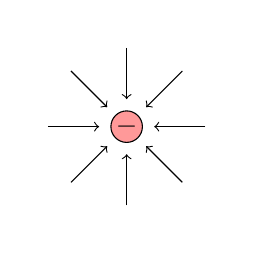
\begin{tikzpicture}
		\filldraw[white] (1.25, 1.25) rectangle (-1.25, -1.25);

		\coordinate (A1) at +(0:1);
		\coordinate (B1) at +(0:0.35);

		\coordinate (A2) at +(45:1);
		\coordinate (B2) at +(45:0.35);

		\coordinate (A3) at +(90:1);
		\coordinate (B3) at +(90:0.35);

		\coordinate (A4) at +(135:1);
		\coordinate (B4) at +(135:0.35);

		\coordinate (A5) at +(180:1);
		\coordinate (B5) at +(180:0.35);

		\coordinate (A6) at +(225:1);
		\coordinate (B6) at +(225:0.35);

		\coordinate (A7) at +(270:1);
		\coordinate (B7) at +(270:0.35);

		\coordinate (A8) at +(315:1);
		\coordinate (B8) at +(315:0.35);

		\draw[->] (A1) -- (B1);
		\draw[->] (A2) -- (B2);
		\draw[->] (A3) -- (B3);
		\draw[->] (A4) -- (B4);
		\draw[->] (A5) -- (B5);
		\draw[->] (A6) -- (B6);
		\draw[->] (A7) -- (B7);
		\draw[->] (A8) -- (B8);

		\filldraw[fill=red!40] (0, 0) circle (0.20);
		\draw (0, 0) node {$-$};
	\end{tikzpicture}
\end{figure}

\end{document}
\usepackage{amsmath}
